\documentclass[1p]{elsarticle_modified}
%\bibliographystyle{elsarticle-num}

%\usepackage[colorlinks]{hyperref}
%\usepackage{abbrmath_seonhwa} %\Abb, \Ascr, \Acal ,\Abf, \Afrak
\usepackage{amsfonts}
\usepackage{amssymb}
\usepackage{amsmath}
\usepackage{amsthm}
\usepackage{scalefnt}
\usepackage{amsbsy}
\usepackage{kotex}
\usepackage{caption}
\usepackage{subfig}
\usepackage{color}
\usepackage{graphicx}
\usepackage{xcolor} %% white, black, red, green, blue, cyan, magenta, yellow
\usepackage{float}
\usepackage{setspace}
\usepackage{hyperref}

\usepackage{tikz}
\usetikzlibrary{arrows}

\usepackage{multirow}
\usepackage{array} % fixed length table
\usepackage{hhline}

%%%%%%%%%%%%%%%%%%%%%
\makeatletter
\renewcommand*\env@matrix[1][\arraystretch]{%
	\edef\arraystretch{#1}%
	\hskip -\arraycolsep
	\let\@ifnextchar\new@ifnextchar
	\array{*\c@MaxMatrixCols c}}
\makeatother %https://tex.stackexchange.com/questions/14071/how-can-i-increase-the-line-spacing-in-a-matrix
%%%%%%%%%%%%%%%

\usepackage[normalem]{ulem}

\newcommand{\msout}[1]{\ifmmode\text{\sout{\ensuremath{#1}}}\else\sout{#1}\fi}
%SOURCE: \msout is \stkout macro in https://tex.stackexchange.com/questions/20609/strikeout-in-math-mode

\newcommand{\cancel}[1]{
	\ifmmode
	{\color{red}\msout{#1}}
	\else
	{\color{red}\sout{#1}}
	\fi
}

\newcommand{\add}[1]{
	{\color{blue}\uwave{#1}}
}

\newcommand{\replace}[2]{
	\ifmmode
	{\color{red}\msout{#1}}{\color{blue}\uwave{#2}}
	\else
	{\color{red}\sout{#1}}{\color{blue}\uwave{#2}}
	\fi
}

\newcommand{\Sol}{\mathcal{S}} %segment
\newcommand{\D}{D} %diagram
\newcommand{\A}{\mathcal{A}} %arc


%%%%%%%%%%%%%%%%%%%%%%%%%%%%%5 test

\def\sl{\operatorname{\textup{SL}}(2,\Cbb)}
\def\psl{\operatorname{\textup{PSL}}(2,\Cbb)}
\def\quan{\mkern 1mu \triangleright \mkern 1mu}

\theoremstyle{definition}
\newtheorem{thm}{Theorem}[section]
\newtheorem{prop}[thm]{Proposition}
\newtheorem{lem}[thm]{Lemma}
\newtheorem{ques}[thm]{Question}
\newtheorem{cor}[thm]{Corollary}
\newtheorem{defn}[thm]{Definition}
\newtheorem{exam}[thm]{Example}
\newtheorem{rmk}[thm]{Remark}
\newtheorem{alg}[thm]{Algorithm}

\newcommand{\I}{\sqrt{-1}}
\begin{document}

%\begin{frontmatter}
%
%\title{Boundary parabolic representations of knots up to 8 crossings}
%
%%% Group authors per affiliation:
%\author{Yunhi Cho} 
%\address{Department of Mathematics, University of Seoul, Seoul, Korea}
%\ead{yhcho@uos.ac.kr}
%
%
%\author{Seonhwa Kim} %\fnref{s_kim}}
%\address{Center for Geometry and Physics, Institute for Basic Science, Pohang, 37673, Korea}
%\ead{ryeona17@ibs.re.kr}
%
%\author{Hyuk Kim}
%\address{Department of Mathematical Sciences, Seoul National University, Seoul 08826, Korea}
%\ead{hyukkim@snu.ac.kr}
%
%\author{Seokbeom Yoon}
%\address{Department of Mathematical Sciences, Seoul National University, Seoul, 08826,  Korea}
%\ead{sbyoon15@snu.ac.kr}
%
%\begin{abstract}
%We find all boundary parabolic representation of knots up to 8 crossings.
%
%\end{abstract}
%\begin{keyword}
%    \MSC[2010] 57M25 
%\end{keyword}
%
%\end{frontmatter}

%\linenumbers
%\tableofcontents
%
\newcommand\colored[1]{\textcolor{white}{\rule[-0.35ex]{0.8em}{1.4ex}}\kern-0.8em\color{red} #1}%
%\newcommand\colored[1]{\textcolor{white}{ #1}\kern-2.17ex	\textcolor{white}{ #1}\kern-1.81ex	\textcolor{white}{ #1}\kern-2.15ex\color{red}#1	}

{\Large $\underline{12a_{0795}~(K12a_{0795})}$}

\setlength{\tabcolsep}{10pt}
\renewcommand{\arraystretch}{1.6}
\vspace{1cm}\begin{tabular}{m{100pt}>{\centering\arraybackslash}m{274pt}}
\multirow{5}{120pt}{
	\centering
	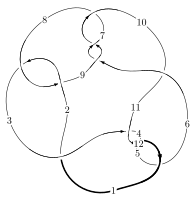
\includegraphics[width=112pt]{../../../GIT/diagram.site/Diagrams/png/1596_12a_0795.png}\\
\ \ \ A knot diagram\footnotemark}&
\allowdisplaybreaks
\textbf{Linearized knot diagam} \\
\cline{2-2}
 &
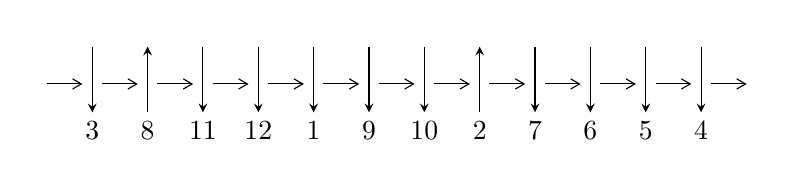
\begin{tikzpicture}[x=20pt, y=17pt]
	% nodes
	\node (C0) at (0, 0) {};
	\node (C1) at (1, 0) {};
	\node (C1U) at (1, +1) {};
	\node (C1D) at (1, -1) {3};

	\node (C2) at (2, 0) {};
	\node (C2U) at (2, +1) {};
	\node (C2D) at (2, -1) {8};

	\node (C3) at (3, 0) {};
	\node (C3U) at (3, +1) {};
	\node (C3D) at (3, -1) {11};

	\node (C4) at (4, 0) {};
	\node (C4U) at (4, +1) {};
	\node (C4D) at (4, -1) {12};

	\node (C5) at (5, 0) {};
	\node (C5U) at (5, +1) {};
	\node (C5D) at (5, -1) {1};

	\node (C6) at (6, 0) {};
	\node (C6U) at (6, +1) {};
	\node (C6D) at (6, -1) {9};

	\node (C7) at (7, 0) {};
	\node (C7U) at (7, +1) {};
	\node (C7D) at (7, -1) {10};

	\node (C8) at (8, 0) {};
	\node (C8U) at (8, +1) {};
	\node (C8D) at (8, -1) {2};

	\node (C9) at (9, 0) {};
	\node (C9U) at (9, +1) {};
	\node (C9D) at (9, -1) {7};

	\node (C10) at (10, 0) {};
	\node (C10U) at (10, +1) {};
	\node (C10D) at (10, -1) {6};

	\node (C11) at (11, 0) {};
	\node (C11U) at (11, +1) {};
	\node (C11D) at (11, -1) {5};

	\node (C12) at (12, 0) {};
	\node (C12U) at (12, +1) {};
	\node (C12D) at (12, -1) {4};
	\node (C13) at (13, 0) {};

	% arrows
	\draw[->,>={angle 60}]
	(C0) edge (C1) (C1) edge (C2) (C2) edge (C3) (C3) edge (C4) (C4) edge (C5) (C5) edge (C6) (C6) edge (C7) (C7) edge (C8) (C8) edge (C9) (C9) edge (C10) (C10) edge (C11) (C11) edge (C12) (C12) edge (C13) ;	\draw[->,>=stealth]
	(C1U) edge (C1D) (C2D) edge (C2U) (C3U) edge (C3D) (C4U) edge (C4D) (C5U) edge (C5D) (C6U) edge (C6D) (C7U) edge (C7D) (C8D) edge (C8U) (C9U) edge (C9D) (C10U) edge (C10D) (C11U) edge (C11D) (C12U) edge (C12D) ;
	\end{tikzpicture} \\
\hhline{~~} \\& 
\textbf{Solving Sequence} \\ \cline{2-2} 
 &
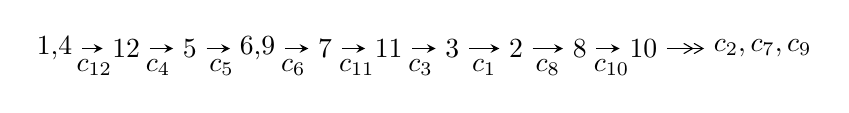
\begin{tikzpicture}[x=23pt, y=7pt]
	% node
	\node (A0) at (-1/8, 0) {1,4};
	\node (A1) at (1, 0) {12};
	\node (A2) at (2, 0) {5};
	\node (A3) at (49/16, 0) {6,9};
	\node (A4) at (33/8, 0) {7};
	\node (A5) at (41/8, 0) {11};
	\node (A6) at (49/8, 0) {3};
	\node (A7) at (57/8, 0) {2};
	\node (A8) at (65/8, 0) {8};
	\node (A9) at (73/8, 0) {10};
	\node (C1) at (1/2, -1) {$c_{12}$};
	\node (C2) at (3/2, -1) {$c_{4}$};
	\node (C3) at (5/2, -1) {$c_{5}$};
	\node (C4) at (29/8, -1) {$c_{6}$};
	\node (C5) at (37/8, -1) {$c_{11}$};
	\node (C6) at (45/8, -1) {$c_{3}$};
	\node (C7) at (53/8, -1) {$c_{1}$};
	\node (C8) at (61/8, -1) {$c_{8}$};
	\node (C9) at (69/8, -1) {$c_{10}$};
	\node (A10) at (11, 0) {$c_{2},c_{7},c_{9}$};

	% edge
	\draw[->,>=stealth]	
	(A0) edge (A1) (A1) edge (A2) (A2) edge (A3) (A3) edge (A4) (A4) edge (A5) (A5) edge (A6) (A6) edge (A7) (A7) edge (A8) (A8) edge (A9) ;
	\draw[->>,>={angle 60}]	
	(A9) edge (A10);
\end{tikzpicture} \\ 

\end{tabular} \\

\footnotetext{
The image of knot diagram is generated by the software ``\textbf{Draw programme}" developed by Andrew Bartholomew(\url{http://www.layer8.co.uk/maths/draw/index.htm\#Running-draw}), where we modified some parts for our purpose(\url{https://github.com/CATsTAILs/LinksPainter}).
}\phantom \\ \newline 
\centering \textbf{Ideals for irreducible components\footnotemark of $X_{\text{par}}$} 
 
\begin{align*}
I^u_{1}&=\langle 
- u^{70}+2 u^{69}+\cdots+b-1,\;2 u^{70}-2 u^{69}+\cdots+a+2,\;u^{71}-2 u^{70}+\cdots+8 u^2-1\rangle \\
I^u_{2}&=\langle 
b,\;u^2+a+1,\;u^3- u^2+2 u-1\rangle \\
\\
\end{align*}
\raggedright * 2 irreducible components of $\dim_{\mathbb{C}}=0$, with total 74 representations.\\
\footnotetext{All coefficients of polynomials are rational numbers. But the coefficients are sometimes approximated in decimal forms when there is not enough margin.}
\newpage
\renewcommand{\arraystretch}{1}
\centering \section*{I. $I^u_{1}= \langle - u^{70}+2 u^{69}+\cdots+b-1,\;2 u^{70}-2 u^{69}+\cdots+a+2,\;u^{71}-2 u^{70}+\cdots+8 u^2-1 \rangle$}
\flushleft \textbf{(i) Arc colorings}\\
\begin{tabular}{m{7pt} m{180pt} m{7pt} m{180pt} }
\flushright $a_{1}=$&$\begin{pmatrix}1\\0\end{pmatrix}$ \\
\flushright $a_{4}=$&$\begin{pmatrix}0\\u\end{pmatrix}$ \\
\flushright $a_{12}=$&$\begin{pmatrix}1\\- u^2\end{pmatrix}$ \\
\flushright $a_{5}=$&$\begin{pmatrix}- u\\u^3+u\end{pmatrix}$ \\
\flushright $a_{6}=$&$\begin{pmatrix}- u^3-2 u\\u^3+u\end{pmatrix}$ \\
\flushright $a_{9}=$&$\begin{pmatrix}-2 u^{70}+2 u^{69}+\cdots-10 u-2\\u^{70}-2 u^{69}+\cdots-14 u^2+1\end{pmatrix}$ \\
\flushright $a_{7}=$&$\begin{pmatrix}- u^{70}+u^{69}+\cdots-10 u-2\\u^{38}+16 u^{36}+\cdots-8 u^3-5 u^2\end{pmatrix}$ \\
\flushright $a_{11}=$&$\begin{pmatrix}u^2+1\\- u^4-2 u^2\end{pmatrix}$ \\
\flushright $a_{3}=$&$\begin{pmatrix}u^5+2 u^3+u\\- u^7-3 u^5-2 u^3+u\end{pmatrix}$ \\
\flushright $a_{2}=$&$\begin{pmatrix}- u^{12}-5 u^{10}-9 u^8-6 u^6+u^2+1\\u^{14}+6 u^{12}+13 u^{10}+10 u^8-2 u^6-4 u^4+u^2\end{pmatrix}$ \\
\flushright $a_{8}=$&$\begin{pmatrix}- u^{58}-25 u^{56}+\cdots-8 u-1\\- u^{70}+2 u^{69}+\cdots- u-1\end{pmatrix}$ \\
\flushright $a_{10}=$&$\begin{pmatrix}- u^{10}-5 u^8-8 u^6-3 u^4+3 u^2+1\\u^{10}+4 u^8+5 u^6-3 u^2\end{pmatrix}$\\&\end{tabular}
\flushleft \textbf{(ii) Obstruction class $= -1$}\\~\\
\flushleft \textbf{(iii) Cusp Shapes $= u^{70}-2 u^{69}+\cdots+5 u-3$}\\~\\
\newpage\renewcommand{\arraystretch}{1}
\flushleft \textbf{(iv) u-Polynomials at the component}\newline \\
\begin{tabular}{m{50pt}|m{274pt}}
Crossings & \hspace{64pt}u-Polynomials at each crossing \\
\hline $$\begin{aligned}c_{1},c_{10}\end{aligned}$$&$\begin{aligned}
&u^{71}+21 u^{70}+\cdots-304 u-64
\end{aligned}$\\
\hline $$\begin{aligned}c_{2},c_{8}\end{aligned}$$&$\begin{aligned}
&u^{71}- u^{70}+\cdots+4 u-8
\end{aligned}$\\
\hline $$\begin{aligned}c_{3},c_{5}\end{aligned}$$&$\begin{aligned}
&u^{71}+2 u^{70}+\cdots-4 u-1
\end{aligned}$\\
\hline $$\begin{aligned}c_{4},c_{11},c_{12}\end{aligned}$$&$\begin{aligned}
&u^{71}-2 u^{70}+\cdots+8 u^2-1
\end{aligned}$\\
\hline $$\begin{aligned}c_{6},c_{7},c_{9}\end{aligned}$$&$\begin{aligned}
&u^{71}-4 u^{70}+\cdots+u-1
\end{aligned}$\\
\hline
\end{tabular}\\~\\
\newpage\renewcommand{\arraystretch}{1}
\flushleft \textbf{(v) Riley Polynomials at the component}\newline \\
\begin{tabular}{m{50pt}|m{274pt}}
Crossings & \hspace{64pt}Riley Polynomials at each crossing \\
\hline $$\begin{aligned}c_{1},c_{10}\end{aligned}$$&$\begin{aligned}
&y^{71}+53 y^{70}+\cdots+216320 y-4096
\end{aligned}$\\
\hline $$\begin{aligned}c_{2},c_{8}\end{aligned}$$&$\begin{aligned}
&y^{71}+21 y^{70}+\cdots-304 y-64
\end{aligned}$\\
\hline $$\begin{aligned}c_{3},c_{5}\end{aligned}$$&$\begin{aligned}
&y^{71}-36 y^{70}+\cdots+16 y-1
\end{aligned}$\\
\hline $$\begin{aligned}c_{4},c_{11},c_{12}\end{aligned}$$&$\begin{aligned}
&y^{71}+60 y^{70}+\cdots+16 y-1
\end{aligned}$\\
\hline $$\begin{aligned}c_{6},c_{7},c_{9}\end{aligned}$$&$\begin{aligned}
&y^{71}-58 y^{70}+\cdots+25 y-1
\end{aligned}$\\
\hline
\end{tabular}\\~\\
\newpage\flushleft \textbf{(vi) Complex Volumes and Cusp Shapes}
$$\begin{array}{c|c|c}  
\text{Solutions to }I^u_{1}& \I (\text{vol} + \sqrt{-1}CS) & \text{Cusp shape}\\
 \hline 
\begin{aligned}
u &= \phantom{-}0.256184 + 1.000660 I \\
a &= -1.44048 - 0.17050 I \\
b &= \phantom{-}0.942819 + 0.538556 I\end{aligned}
 & \phantom{-}3.71024 + 2.74767 I & \phantom{-0.000000 } 0 \\ \hline\begin{aligned}
u &= \phantom{-}0.256184 - 1.000660 I \\
a &= -1.44048 + 0.17050 I \\
b &= \phantom{-}0.942819 - 0.538556 I\end{aligned}
 & \phantom{-}3.71024 - 2.74767 I & \phantom{-0.000000 } 0 \\ \hline\begin{aligned}
u &= \phantom{-}0.329944 + 1.015460 I \\
a &= \phantom{-}1.74724 + 0.53409 I \\
b &= -0.84648 - 1.80456 I\end{aligned}
 & -0.89927 + 6.92261 I & \phantom{-0.000000 } 0 \\ \hline\begin{aligned}
u &= \phantom{-}0.329944 - 1.015460 I \\
a &= \phantom{-}1.74724 - 0.53409 I \\
b &= -0.84648 + 1.80456 I\end{aligned}
 & -0.89927 - 6.92261 I & \phantom{-0.000000 } 0 \\ \hline\begin{aligned}
u &= -0.214843 + 1.069620 I \\
a &= \phantom{-}1.85403 - 0.34171 I \\
b &= -0.62007 + 1.89231 I\end{aligned}
 & \phantom{-}0.438100 - 1.074520 I & \phantom{-0.000000 } 0 \\ \hline\begin{aligned}
u &= -0.214843 - 1.069620 I \\
a &= \phantom{-}1.85403 + 0.34171 I \\
b &= -0.62007 - 1.89231 I\end{aligned}
 & \phantom{-}0.438100 + 1.074520 I & \phantom{-0.000000 } 0 \\ \hline\begin{aligned}
u &= \phantom{-}0.179274 + 1.163920 I \\
a &= \phantom{-}1.196860 - 0.319658 I \\
b &= -0.042857 + 0.336767 I\end{aligned}
 & \phantom{-}0.86953 - 1.32939 I & \phantom{-0.000000 } 0 \\ \hline\begin{aligned}
u &= \phantom{-}0.179274 - 1.163920 I \\
a &= \phantom{-}1.196860 + 0.319658 I \\
b &= -0.042857 - 0.336767 I\end{aligned}
 & \phantom{-}0.86953 + 1.32939 I & \phantom{-0.000000 } 0 \\ \hline\begin{aligned}
u &= -0.217571 + 0.785287 I \\
a &= -1.245700 - 0.372469 I \\
b &= \phantom{-}1.125800 - 0.040746 I\end{aligned}
 & \phantom{-}3.94493 + 2.68423 I & -3.68030 - 4.11188 I \\ \hline\begin{aligned}
u &= -0.217571 - 0.785287 I \\
a &= -1.245700 + 0.372469 I \\
b &= \phantom{-}1.125800 + 0.040746 I\end{aligned}
 & \phantom{-}3.94493 - 2.68423 I & -3.68030 + 4.11188 I\\
 \hline 
 \end{array}$$\newpage$$\begin{array}{c|c|c}  
\text{Solutions to }I^u_{1}& \I (\text{vol} + \sqrt{-1}CS) & \text{Cusp shape}\\
 \hline 
\begin{aligned}
u &= \phantom{-}0.791627 + 0.174417 I \\
a &= -0.70746 + 3.50167 I \\
b &= \phantom{-}1.24243 - 2.17476 I\end{aligned}
 & -3.48296 - 11.07580 I & -12.4369 + 7.9989 I \\ \hline\begin{aligned}
u &= \phantom{-}0.791627 - 0.174417 I \\
a &= -0.70746 - 3.50167 I \\
b &= \phantom{-}1.24243 + 2.17476 I\end{aligned}
 & -3.48296 + 11.07580 I & -12.4369 - 7.9989 I \\ \hline\begin{aligned}
u &= -0.324904 + 0.736311 I \\
a &= \phantom{-}0.816203 + 0.458100 I \\
b &= -0.792190 - 0.999424 I\end{aligned}
 & -0.33299 + 6.68944 I & -8.75568 - 6.96134 I \\ \hline\begin{aligned}
u &= -0.324904 - 0.736311 I \\
a &= \phantom{-}0.816203 - 0.458100 I \\
b &= -0.792190 + 0.999424 I\end{aligned}
 & -0.33299 - 6.68944 I & -8.75568 + 6.96134 I \\ \hline\begin{aligned}
u &= \phantom{-}0.801438 + 0.059793 I \\
a &= -1.39728 + 1.51429 I \\
b &= \phantom{-}1.55766 - 0.93488 I\end{aligned}
 & -10.39180 - 4.18324 I & -17.6640 + 4.0027 I \\ \hline\begin{aligned}
u &= \phantom{-}0.801438 - 0.059793 I \\
a &= -1.39728 - 1.51429 I \\
b &= \phantom{-}1.55766 + 0.93488 I\end{aligned}
 & -10.39180 + 4.18324 I & -17.6640 - 4.0027 I \\ \hline\begin{aligned}
u &= \phantom{-}0.767734 + 0.173295 I \\
a &= \phantom{-}1.48648 - 2.41574 I \\
b &= -1.20346 + 1.04399 I\end{aligned}
 & \phantom{-}1.17708 - 6.66958 I & -8.37292 + 6.44479 I \\ \hline\begin{aligned}
u &= \phantom{-}0.767734 - 0.173295 I \\
a &= \phantom{-}1.48648 + 2.41574 I \\
b &= -1.20346 - 1.04399 I\end{aligned}
 & \phantom{-}1.17708 + 6.66958 I & -8.37292 - 6.44479 I \\ \hline\begin{aligned}
u &= -0.756173 + 0.159399 I \\
a &= -1.18126 - 3.65137 I \\
b &= \phantom{-}1.52619 + 2.22298 I\end{aligned}
 & -2.23215 + 4.83532 I & -11.48650 - 4.26666 I \\ \hline\begin{aligned}
u &= -0.756173 - 0.159399 I \\
a &= -1.18126 + 3.65137 I \\
b &= \phantom{-}1.52619 - 2.22298 I\end{aligned}
 & -2.23215 - 4.83532 I & -11.48650 + 4.26666 I\\
 \hline 
 \end{array}$$\newpage$$\begin{array}{c|c|c}  
\text{Solutions to }I^u_{1}& \I (\text{vol} + \sqrt{-1}CS) & \text{Cusp shape}\\
 \hline 
\begin{aligned}
u &= \phantom{-}0.347096 + 1.197000 I \\
a &= \phantom{-}0.890138 - 0.346320 I \\
b &= -1.26266 - 1.32210 I\end{aligned}
 & -6.90568 + 0.03158 I & \phantom{-0.000000 } 0 \\ \hline\begin{aligned}
u &= \phantom{-}0.347096 - 1.197000 I \\
a &= \phantom{-}0.890138 + 0.346320 I \\
b &= -1.26266 + 1.32210 I\end{aligned}
 & -6.90568 - 0.03158 I & \phantom{-0.000000 } 0 \\ \hline\begin{aligned}
u &= \phantom{-}0.733221 + 0.158026 I \\
a &= -1.82401 + 0.88157 I \\
b &= \phantom{-}0.636704 - 0.077125 I\end{aligned}
 & -1.87111 - 2.10145 I & -11.67107 + 3.54361 I \\ \hline\begin{aligned}
u &= \phantom{-}0.733221 - 0.158026 I \\
a &= -1.82401 - 0.88157 I \\
b &= \phantom{-}0.636704 + 0.077125 I\end{aligned}
 & -1.87111 + 2.10145 I & -11.67107 - 3.54361 I \\ \hline\begin{aligned}
u &= -0.723605 + 0.189746 I \\
a &= \phantom{-}1.73646 + 1.99125 I \\
b &= -1.28817 - 0.74944 I\end{aligned}
 & \phantom{-}1.83396 + 0.92082 I & -6.84757 - 1.21767 I \\ \hline\begin{aligned}
u &= -0.723605 - 0.189746 I \\
a &= \phantom{-}1.73646 - 1.99125 I \\
b &= -1.28817 + 0.74944 I\end{aligned}
 & \phantom{-}1.83396 - 0.92082 I & -6.84757 + 1.21767 I \\ \hline\begin{aligned}
u &= -0.747959\phantom{ +0.000000I} \\
a &= -3.24996\phantom{ +0.000000I} \\
b &= \phantom{-}2.66245\phantom{ +0.000000I}\end{aligned}
 & -6.09275\phantom{ +0.000000I} & -15.2180\phantom{ +0.000000I} \\ \hline\begin{aligned}
u &= \phantom{-}0.742764 + 0.034256 I \\
a &= -0.00879 - 1.63305 I \\
b &= -0.299685 + 0.720499 I\end{aligned}
 & -4.20092 - 2.01610 I & -15.1041 + 4.5782 I \\ \hline\begin{aligned}
u &= \phantom{-}0.742764 - 0.034256 I \\
a &= -0.00879 + 1.63305 I \\
b &= -0.299685 - 0.720499 I\end{aligned}
 & -4.20092 + 2.01610 I & -15.1041 - 4.5782 I \\ \hline\begin{aligned}
u &= -0.697910 + 0.237511 I \\
a &= -1.97426 - 0.37324 I \\
b &= \phantom{-}0.650196 - 0.355443 I\end{aligned}
 & -2.02822 - 2.95146 I & -11.59106 + 2.08454 I\\
 \hline 
 \end{array}$$\newpage$$\begin{array}{c|c|c}  
\text{Solutions to }I^u_{1}& \I (\text{vol} + \sqrt{-1}CS) & \text{Cusp shape}\\
 \hline 
\begin{aligned}
u &= -0.697910 - 0.237511 I \\
a &= -1.97426 + 0.37324 I \\
b &= \phantom{-}0.650196 + 0.355443 I\end{aligned}
 & -2.02822 + 2.95146 I & -11.59106 - 2.08454 I \\ \hline\begin{aligned}
u &= -0.111577 + 1.260490 I \\
a &= -0.973741 + 0.037777 I \\
b &= -0.005497 - 0.653120 I\end{aligned}
 & \phantom{-}4.01768 + 1.95795 I & \phantom{-0.000000 } 0 \\ \hline\begin{aligned}
u &= -0.111577 - 1.260490 I \\
a &= -0.973741 - 0.037777 I \\
b &= -0.005497 + 0.653120 I\end{aligned}
 & \phantom{-}4.01768 - 1.95795 I & \phantom{-0.000000 } 0 \\ \hline\begin{aligned}
u &= \phantom{-}0.093225 + 0.721635 I \\
a &= \phantom{-}1.274690 + 0.098830 I \\
b &= -0.760475 + 0.967960 I\end{aligned}
 & \phantom{-}0.538881 - 1.251930 I & -6.70748 + 0.95320 I \\ \hline\begin{aligned}
u &= \phantom{-}0.093225 - 0.721635 I \\
a &= \phantom{-}1.274690 - 0.098830 I \\
b &= -0.760475 - 0.967960 I\end{aligned}
 & \phantom{-}0.538881 + 1.251930 I & -6.70748 - 0.95320 I \\ \hline\begin{aligned}
u &= \phantom{-}0.293715 + 1.240310 I \\
a &= -0.461247 - 0.815444 I \\
b &= \phantom{-}0.109258 + 0.796307 I\end{aligned}
 & -0.49943 - 1.72973 I & \phantom{-0.000000 } 0 \\ \hline\begin{aligned}
u &= \phantom{-}0.293715 - 1.240310 I \\
a &= -0.461247 + 0.815444 I \\
b &= \phantom{-}0.109258 - 0.796307 I\end{aligned}
 & -0.49943 + 1.72973 I & \phantom{-0.000000 } 0 \\ \hline\begin{aligned}
u &= -0.309231 + 1.263960 I \\
a &= \phantom{-}0.71727 + 1.79747 I \\
b &= -2.66465 + 0.70550 I\end{aligned}
 & -2.17852 + 3.81797 I & \phantom{-0.000000 } 0 \\ \hline\begin{aligned}
u &= -0.309231 - 1.263960 I \\
a &= \phantom{-}0.71727 - 1.79747 I \\
b &= -2.66465 - 0.70550 I\end{aligned}
 & -2.17852 - 3.81797 I & \phantom{-0.000000 } 0 \\ \hline\begin{aligned}
u &= -0.246621 + 1.292500 I \\
a &= -0.081651 - 0.489646 I \\
b &= \phantom{-}0.688163 - 0.243775 I\end{aligned}
 & \phantom{-}2.61245 + 3.17474 I & \phantom{-0.000000 } 0\\
 \hline 
 \end{array}$$\newpage$$\begin{array}{c|c|c}  
\text{Solutions to }I^u_{1}& \I (\text{vol} + \sqrt{-1}CS) & \text{Cusp shape}\\
 \hline 
\begin{aligned}
u &= -0.246621 - 1.292500 I \\
a &= -0.081651 + 0.489646 I \\
b &= \phantom{-}0.688163 + 0.243775 I\end{aligned}
 & \phantom{-}2.61245 - 3.17474 I & \phantom{-0.000000 } 0 \\ \hline\begin{aligned}
u &= \phantom{-}0.312288 + 1.286840 I \\
a &= \phantom{-}0.832695 + 0.953099 I \\
b &= \phantom{-}0.466349 - 0.620225 I\end{aligned}
 & -0.08510 - 5.83054 I & \phantom{-0.000000 } 0 \\ \hline\begin{aligned}
u &= \phantom{-}0.312288 - 1.286840 I \\
a &= \phantom{-}0.832695 - 0.953099 I \\
b &= \phantom{-}0.466349 + 0.620225 I\end{aligned}
 & -0.08510 + 5.83054 I & \phantom{-0.000000 } 0 \\ \hline\begin{aligned}
u &= \phantom{-}0.350571 + 1.300740 I \\
a &= -0.51714 - 1.46183 I \\
b &= -1.72983 + 0.54565 I\end{aligned}
 & -6.14537 - 8.33234 I & \phantom{-0.000000 } 0 \\ \hline\begin{aligned}
u &= \phantom{-}0.350571 - 1.300740 I \\
a &= -0.51714 + 1.46183 I \\
b &= -1.72983 - 0.54565 I\end{aligned}
 & -6.14537 + 8.33234 I & \phantom{-0.000000 } 0 \\ \hline\begin{aligned}
u &= -0.632866\phantom{ +0.000000I} \\
a &= \phantom{-}0.755852\phantom{ +0.000000I} \\
b &= -0.593534\phantom{ +0.000000I}\end{aligned}
 & -1.44345\phantom{ +0.000000I} & -6.17470\phantom{ +0.000000I} \\ \hline\begin{aligned}
u &= -0.161984 + 1.369530 I \\
a &= \phantom{-}0.826573 + 0.609366 I \\
b &= \phantom{-}0.182639 + 0.542628 I\end{aligned}
 & \phantom{-}0.43014 + 3.75727 I & \phantom{-0.000000 } 0 \\ \hline\begin{aligned}
u &= -0.161984 - 1.369530 I \\
a &= \phantom{-}0.826573 - 0.609366 I \\
b &= \phantom{-}0.182639 - 0.542628 I\end{aligned}
 & \phantom{-}0.43014 - 3.75727 I & \phantom{-0.000000 } 0 \\ \hline\begin{aligned}
u &= \phantom{-}0.310198 + 1.356630 I \\
a &= \phantom{-}0.60405 - 1.33113 I \\
b &= -0.858121 + 0.380258 I\end{aligned}
 & \phantom{-}2.90857 - 5.89514 I & \phantom{-0.000000 } 0 \\ \hline\begin{aligned}
u &= \phantom{-}0.310198 - 1.356630 I \\
a &= \phantom{-}0.60405 + 1.33113 I \\
b &= -0.858121 - 0.380258 I\end{aligned}
 & \phantom{-}2.90857 + 5.89514 I & \phantom{-0.000000 } 0\\
 \hline 
 \end{array}$$\newpage$$\begin{array}{c|c|c}  
\text{Solutions to }I^u_{1}& \I (\text{vol} + \sqrt{-1}CS) & \text{Cusp shape}\\
 \hline 
\begin{aligned}
u &= -0.457320 + 0.399866 I \\
a &= -0.876469 - 0.014419 I \\
b &= -0.207572 - 0.853124 I\end{aligned}
 & -5.04352 + 1.61644 I & -14.6425 - 4.5743 I \\ \hline\begin{aligned}
u &= -0.457320 - 0.399866 I \\
a &= -0.876469 + 0.014419 I \\
b &= -0.207572 + 0.853124 I\end{aligned}
 & -5.04352 - 1.61644 I & -14.6425 + 4.5743 I \\ \hline\begin{aligned}
u &= -0.319562 + 1.359040 I \\
a &= -1.46931 + 2.12621 I \\
b &= -2.00071 - 2.27701 I\end{aligned}
 & \phantom{-}2.55975 + 8.73487 I & \phantom{-0.000000 } 0 \\ \hline\begin{aligned}
u &= -0.319562 - 1.359040 I \\
a &= -1.46931 - 2.12621 I \\
b &= -2.00071 + 2.27701 I\end{aligned}
 & \phantom{-}2.55975 - 8.73487 I & \phantom{-0.000000 } 0 \\ \hline\begin{aligned}
u &= -0.302482 + 1.367500 I \\
a &= \phantom{-}0.25531 - 1.81957 I \\
b &= \phantom{-}1.60307 + 0.95919 I\end{aligned}
 & \phantom{-}6.75117 + 4.65324 I & \phantom{-0.000000 } 0 \\ \hline\begin{aligned}
u &= -0.302482 - 1.367500 I \\
a &= \phantom{-}0.25531 + 1.81957 I \\
b &= \phantom{-}1.60307 - 0.95919 I\end{aligned}
 & \phantom{-}6.75117 - 4.65324 I & \phantom{-0.000000 } 0 \\ \hline\begin{aligned}
u &= \phantom{-}0.323439 + 1.366540 I \\
a &= \phantom{-}0.49653 + 1.92085 I \\
b &= \phantom{-}1.43211 - 1.25712 I\end{aligned}
 & \phantom{-}6.04049 - 10.62110 I & \phantom{-0.000000 } 0 \\ \hline\begin{aligned}
u &= \phantom{-}0.323439 - 1.366540 I \\
a &= \phantom{-}0.49653 - 1.92085 I \\
b &= \phantom{-}1.43211 + 1.25712 I\end{aligned}
 & \phantom{-}6.04049 + 10.62110 I & \phantom{-0.000000 } 0 \\ \hline\begin{aligned}
u &= \phantom{-}0.006893 + 1.406310 I \\
a &= \phantom{-}0.364284 - 0.865963 I \\
b &= \phantom{-}1.82585 - 0.65702 I\end{aligned}
 & \phantom{-}6.91128 - 1.42136 I & \phantom{-0.000000 } 0 \\ \hline\begin{aligned}
u &= \phantom{-}0.006893 - 1.406310 I \\
a &= \phantom{-}0.364284 + 0.865963 I \\
b &= \phantom{-}1.82585 + 0.65702 I\end{aligned}
 & \phantom{-}6.91128 + 1.42136 I & \phantom{-0.000000 } 0\\
 \hline 
 \end{array}$$\newpage$$\begin{array}{c|c|c}  
\text{Solutions to }I^u_{1}& \I (\text{vol} + \sqrt{-1}CS) & \text{Cusp shape}\\
 \hline 
\begin{aligned}
u &= -0.282957 + 1.379610 I \\
a &= \phantom{-}0.840598 + 1.131810 I \\
b &= -0.867253 + 0.022284 I\end{aligned}
 & \phantom{-}3.08119 + 0.61059 I & \phantom{-0.000000 } 0 \\ \hline\begin{aligned}
u &= -0.282957 - 1.379610 I \\
a &= \phantom{-}0.840598 - 1.131810 I \\
b &= -0.867253 - 0.022284 I\end{aligned}
 & \phantom{-}3.08119 - 0.61059 I & \phantom{-0.000000 } 0 \\ \hline\begin{aligned}
u &= \phantom{-}0.334719 + 1.370140 I \\
a &= -1.57757 - 1.91835 I \\
b &= -1.55721 + 2.29709 I\end{aligned}
 & \phantom{-}1.3962 - 15.1466 I & \phantom{-0.000000 } 0 \\ \hline\begin{aligned}
u &= \phantom{-}0.334719 - 1.370140 I \\
a &= -1.57757 + 1.91835 I \\
b &= -1.55721 - 2.29709 I\end{aligned}
 & \phantom{-}1.3962 + 15.1466 I & \phantom{-0.000000 } 0 \\ \hline\begin{aligned}
u &= -0.01386 + 1.41878 I \\
a &= -0.569707 + 0.076935 I \\
b &= -1.93745 - 0.20438 I\end{aligned}
 & \phantom{-}10.58420 + 3.03649 I & \phantom{-0.000000 } 0 \\ \hline\begin{aligned}
u &= -0.01386 - 1.41878 I \\
a &= -0.569707 - 0.076935 I \\
b &= -1.93745 + 0.20438 I\end{aligned}
 & \phantom{-}10.58420 - 3.03649 I & \phantom{-0.000000 } 0 \\ \hline\begin{aligned}
u &= -0.03263 + 1.42756 I \\
a &= \phantom{-}0.369062 + 0.657493 I \\
b &= \phantom{-}1.61604 + 1.00344 I\end{aligned}
 & \phantom{-}6.40163 + 7.44140 I & \phantom{-0.000000 } 0 \\ \hline\begin{aligned}
u &= -0.03263 - 1.42756 I \\
a &= \phantom{-}0.369062 - 0.657493 I \\
b &= \phantom{-}1.61604 - 1.00344 I\end{aligned}
 & \phantom{-}6.40163 - 7.44140 I & \phantom{-0.000000 } 0 \\ \hline\begin{aligned}
u &= -0.226398 + 0.239535 I \\
a &= \phantom{-}0.930119 - 0.695460 I \\
b &= \phantom{-}0.086502 + 0.441868 I\end{aligned}
 & -0.325148 + 0.797487 I & -7.87828 - 8.56231 I \\ \hline\begin{aligned}
u &= -0.226398 - 0.239535 I \\
a &= \phantom{-}0.930119 + 0.695460 I \\
b &= \phantom{-}0.086502 - 0.441868 I\end{aligned}
 & -0.325148 - 0.797487 I & -7.87828 + 8.56231 I\\
 \hline 
 \end{array}$$\newpage$$\begin{array}{c|c|c}  
\text{Solutions to }I^u_{1}& \I (\text{vol} + \sqrt{-1}CS) & \text{Cusp shape}\\
 \hline 
\begin{aligned}
u &= \phantom{-}0.231421\phantom{ +0.000000I} \\
a &= -3.37094\phantom{ +0.000000I} \\
b &= -0.563822\phantom{ +0.000000I}\end{aligned}
 & -2.02563\phantom{ +0.000000I} & -2.73450\phantom{ +0.000000I}\\
 \hline 
 \end{array}$$\newpage\newpage\renewcommand{\arraystretch}{1}
\centering \section*{II. $I^u_{2}= \langle b,\;u^2+a+1,\;u^3- u^2+2 u-1 \rangle$}
\flushleft \textbf{(i) Arc colorings}\\
\begin{tabular}{m{7pt} m{180pt} m{7pt} m{180pt} }
\flushright $a_{1}=$&$\begin{pmatrix}1\\0\end{pmatrix}$ \\
\flushright $a_{4}=$&$\begin{pmatrix}0\\u\end{pmatrix}$ \\
\flushright $a_{12}=$&$\begin{pmatrix}1\\- u^2\end{pmatrix}$ \\
\flushright $a_{5}=$&$\begin{pmatrix}- u\\u^2- u+1\end{pmatrix}$ \\
\flushright $a_{6}=$&$\begin{pmatrix}- u^2-1\\u^2- u+1\end{pmatrix}$ \\
\flushright $a_{9}=$&$\begin{pmatrix}- u^2-1\\0\end{pmatrix}$ \\
\flushright $a_{7}=$&$\begin{pmatrix}-2 u^2-2\\u^2- u+1\end{pmatrix}$ \\
\flushright $a_{11}=$&$\begin{pmatrix}u^2+1\\- u^2+u-1\end{pmatrix}$ \\
\flushright $a_{3}=$&$\begin{pmatrix}1\\0\end{pmatrix}$ \\
\flushright $a_{2}=$&$\begin{pmatrix}1\\0\end{pmatrix}$ \\
\flushright $a_{8}=$&$\begin{pmatrix}- u^2-1\\0\end{pmatrix}$ \\
\flushright $a_{10}=$&$\begin{pmatrix}u^2+1\\- u^2+u-1\end{pmatrix}$\\&\end{tabular}
\flushleft \textbf{(ii) Obstruction class $= 1$}\\~\\
\flushleft \textbf{(iii) Cusp Shapes $= -5 u^2+4 u-16$}\\~\\
\newpage\renewcommand{\arraystretch}{1}
\flushleft \textbf{(iv) u-Polynomials at the component}\newline \\
\begin{tabular}{m{50pt}|m{274pt}}
Crossings & \hspace{64pt}u-Polynomials at each crossing \\
\hline $$\begin{aligned}c_{1},c_{2},c_{8}\\c_{10}\end{aligned}$$&$\begin{aligned}
&u^3
\end{aligned}$\\
\hline $$\begin{aligned}c_{3},c_{5}\end{aligned}$$&$\begin{aligned}
&u^3- u^2+1
\end{aligned}$\\
\hline $$\begin{aligned}c_{4}\end{aligned}$$&$\begin{aligned}
&u^3+u^2+2 u+1
\end{aligned}$\\
\hline $$\begin{aligned}c_{6},c_{7}\end{aligned}$$&$\begin{aligned}
&(u-1)^3
\end{aligned}$\\
\hline $$\begin{aligned}c_{9}\end{aligned}$$&$\begin{aligned}
&(u+1)^3
\end{aligned}$\\
\hline $$\begin{aligned}c_{11},c_{12}\end{aligned}$$&$\begin{aligned}
&u^3- u^2+2 u-1
\end{aligned}$\\
\hline
\end{tabular}\\~\\
\newpage\renewcommand{\arraystretch}{1}
\flushleft \textbf{(v) Riley Polynomials at the component}\newline \\
\begin{tabular}{m{50pt}|m{274pt}}
Crossings & \hspace{64pt}Riley Polynomials at each crossing \\
\hline $$\begin{aligned}c_{1},c_{2},c_{8}\\c_{10}\end{aligned}$$&$\begin{aligned}
&y^3
\end{aligned}$\\
\hline $$\begin{aligned}c_{3},c_{5}\end{aligned}$$&$\begin{aligned}
&y^3- y^2+2 y-1
\end{aligned}$\\
\hline $$\begin{aligned}c_{4},c_{11},c_{12}\end{aligned}$$&$\begin{aligned}
&y^3+3 y^2+2 y-1
\end{aligned}$\\
\hline $$\begin{aligned}c_{6},c_{7},c_{9}\end{aligned}$$&$\begin{aligned}
&(y-1)^3
\end{aligned}$\\
\hline
\end{tabular}\\~\\
\newpage\flushleft \textbf{(vi) Complex Volumes and Cusp Shapes}
$$\begin{array}{c|c|c}  
\text{Solutions to }I^u_{2}& \I (\text{vol} + \sqrt{-1}CS) & \text{Cusp shape}\\
 \hline 
\begin{aligned}
u &= \phantom{-}0.215080 + 1.307140 I \\
a &= \phantom{-}0.662359 - 0.562280 I \\
b &= \phantom{-0.000000 } 0\end{aligned}
 & \phantom{-}1.37919 - 2.82812 I & -6.82789 + 2.41717 I \\ \hline\begin{aligned}
u &= \phantom{-}0.215080 - 1.307140 I \\
a &= \phantom{-}0.662359 + 0.562280 I \\
b &= \phantom{-0.000000 } 0\end{aligned}
 & \phantom{-}1.37919 + 2.82812 I & -6.82789 - 2.41717 I \\ \hline\begin{aligned}
u &= \phantom{-}0.569840\phantom{ +0.000000I} \\
a &= -1.32472\phantom{ +0.000000I} \\
b &= \phantom{-0.000000 } 0\end{aligned}
 & -2.75839\phantom{ +0.000000I} & -15.3440\phantom{ +0.000000I}\\
 \hline 
 \end{array}$$\newpage
\newpage\renewcommand{\arraystretch}{1}
\centering \section*{ III. u-Polynomials}
\begin{tabular}{m{50pt}|m{274pt}}
Crossings & \hspace{64pt}u-Polynomials at each crossing \\
\hline $$\begin{aligned}c_{1},c_{10}\end{aligned}$$&$\begin{aligned}
&u^3(u^{71}+21 u^{70}+\cdots-304 u-64)
\end{aligned}$\\
\hline $$\begin{aligned}c_{2},c_{8}\end{aligned}$$&$\begin{aligned}
&u^3(u^{71}- u^{70}+\cdots+4 u-8)
\end{aligned}$\\
\hline $$\begin{aligned}c_{3},c_{5}\end{aligned}$$&$\begin{aligned}
&(u^3- u^2+1)(u^{71}+2 u^{70}+\cdots-4 u-1)
\end{aligned}$\\
\hline $$\begin{aligned}c_{4}\end{aligned}$$&$\begin{aligned}
&(u^3+u^2+2 u+1)(u^{71}-2 u^{70}+\cdots+8 u^2-1)
\end{aligned}$\\
\hline $$\begin{aligned}c_{6},c_{7}\end{aligned}$$&$\begin{aligned}
&((u-1)^3)(u^{71}-4 u^{70}+\cdots+u-1)
\end{aligned}$\\
\hline $$\begin{aligned}c_{9}\end{aligned}$$&$\begin{aligned}
&((u+1)^3)(u^{71}-4 u^{70}+\cdots+u-1)
\end{aligned}$\\
\hline $$\begin{aligned}c_{11},c_{12}\end{aligned}$$&$\begin{aligned}
&(u^3- u^2+2 u-1)(u^{71}-2 u^{70}+\cdots+8 u^2-1)
\end{aligned}$\\
\hline
\end{tabular}\newpage\renewcommand{\arraystretch}{1}
\centering \section*{ IV. Riley Polynomials}
\begin{tabular}{m{50pt}|m{274pt}}
Crossings & \hspace{64pt}Riley Polynomials at each crossing \\
\hline $$\begin{aligned}c_{1},c_{10}\end{aligned}$$&$\begin{aligned}
&y^3(y^{71}+53 y^{70}+\cdots+216320 y-4096)
\end{aligned}$\\
\hline $$\begin{aligned}c_{2},c_{8}\end{aligned}$$&$\begin{aligned}
&y^3(y^{71}+21 y^{70}+\cdots-304 y-64)
\end{aligned}$\\
\hline $$\begin{aligned}c_{3},c_{5}\end{aligned}$$&$\begin{aligned}
&(y^3- y^2+2 y-1)(y^{71}-36 y^{70}+\cdots+16 y-1)
\end{aligned}$\\
\hline $$\begin{aligned}c_{4},c_{11},c_{12}\end{aligned}$$&$\begin{aligned}
&(y^3+3 y^2+2 y-1)(y^{71}+60 y^{70}+\cdots+16 y-1)
\end{aligned}$\\
\hline $$\begin{aligned}c_{6},c_{7},c_{9}\end{aligned}$$&$\begin{aligned}
&((y-1)^3)(y^{71}-58 y^{70}+\cdots+25 y-1)
\end{aligned}$\\
\hline
\end{tabular}
\vskip 2pc
\end{document}